\section{Pessimistic Concurrency Control} \label{sec:pessimistic}

To provide a baseline against which to compare the performance of HTM, we
implemented two different forms of traditional, software-based pessimistic
concurrency control protocols: a lock manager and spin locks.

\subsection{Lock Manager}

Traditional locking schemes make use of a lock manager, which arbitrates access
to records in the key-value store by granting locks to requesting transactions.
In our implementation, each key-value pair has its own lock. (Some lock managers
maintain coarser-grained locks, protecting groups of keys, to decrease locking
overhead; we did not attempt this optimization in the course of this project.)
The lock manager consists of a lock table hashed on keys. Each lock record
includes a list of transactions waiting to acquire the lock. A transaction may
only access a given key-value pair once it has requested and been granted the
appropriate lock, which prevents conflicting concurrent operations.

When a process requests a lock, the lock manager grants the request if it is
compatible with the lock's current state. When the transaction currently holding
the lock releases it, the lock manager grants the lock to the transaction at the
head of the waiting queue for that lock.

We experimented with both simple mutex locks, in which every lock is either free
or locked, and read/write locks, in which each lock has a ``mode'' (read, write,
or free), and multiple readers may hold the lock simultaneously in ``read''
mode. We found that read/write locks imposed enormous overhead and were not
competitive with any other concurrency control schemes, so we omitted them from
our tests.

For static read/write sets, we prevented deadlocks by enforcing an ordering in
which a transaction may request locks, which ensures that no circular
dependencies between transactions waiting on locks may occur. For dynamic
read/write sets, we implemented a very simple scheme to break deadlocks
based on timeouts.\\

\subsection{Spin Locks}

A spin lock is simply a memory word representing a lock, which can be acquired
via an atomic test-and-set primitive. If a transaction attempts test-and-set but
it fails because the lock is already held, the transaction \textit{spins}, or
repeatedly attempts to grab the lock until it succeeds.

We implemented two different spin lock-based schemes. In one version, there is a
single spin lock for the entire table, serializing all transactions. We call
this the ``simple spin lock'' implementation. The second implementation uses
fine-grained locks, much like the lock manager scheme: each key is protected by
a single spin lock. In this scheme, deadlock prevention is implemented exactly
as in the lock table scheme.

By avoiding the extra work of going through the manager, spin locks can
potentially be faster. However, the obvious disadvantage of spin locks is that
they require ``busy waiting'': when a transaction spins while waiting for a
lock, it is using CPU time without doing any useful work. This is primarily a
problem in systems with high contention, where it is likely that multiple
transactions will want to access the same key-value pair at the same time. Prior
work \citep{tran2010} has suggested, based on an HTM simulator, that TM peforms
well under low-contection workloads, whereas spinlocks work better under
high-contention workloads. We investigated how valid this observation is in a
real-world HTM implementation.

%Time required to access a given number of objects using different concurrency
%control protocols, based on their simulation, is shown in \Cref{fig:overhead}. 

% jarulraj: Removed figure for now -- not sure if we can use it
%\begin{figure}[h!] \centering
%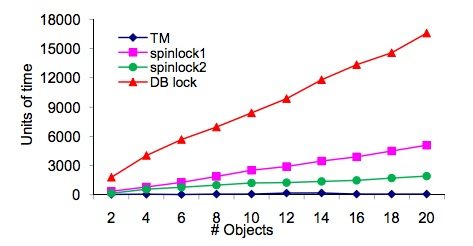
\includegraphics[width=0.45\textwidth]{figure/overhead.jpg} \caption{Overhead
%of different concurrency control protocols under low contention workloads
%\citep{tran2010}.} \label{fig:overhead} \end{figure}
